\documentclass[11pt, a4paper]{article}\usepackage[]{graphicx}\usepackage[]{xcolor}
% maxwidth is the original width if it is less than linewidth
% otherwise use linewidth (to make sure the graphics do not exceed the margin)
\makeatletter
\def\maxwidth{ %
  \ifdim\Gin@nat@width>\linewidth
    \linewidth
  \else
    \Gin@nat@width
  \fi
}
\makeatother

\definecolor{fgcolor}{rgb}{0.345, 0.345, 0.345}
\newcommand{\hlnum}[1]{\textcolor[rgb]{0.686,0.059,0.569}{#1}}%
\newcommand{\hlsng}[1]{\textcolor[rgb]{0.192,0.494,0.8}{#1}}%
\newcommand{\hlcom}[1]{\textcolor[rgb]{0.678,0.584,0.686}{\textit{#1}}}%
\newcommand{\hlopt}[1]{\textcolor[rgb]{0,0,0}{#1}}%
\newcommand{\hldef}[1]{\textcolor[rgb]{0.345,0.345,0.345}{#1}}%
\newcommand{\hlkwa}[1]{\textcolor[rgb]{0.161,0.373,0.58}{\textbf{#1}}}%
\newcommand{\hlkwb}[1]{\textcolor[rgb]{0.69,0.353,0.396}{#1}}%
\newcommand{\hlkwc}[1]{\textcolor[rgb]{0.333,0.667,0.333}{#1}}%
\newcommand{\hlkwd}[1]{\textcolor[rgb]{0.737,0.353,0.396}{\textbf{#1}}}%
\let\hlipl\hlkwb

\usepackage{framed}
\makeatletter
\newenvironment{kframe}{%
 \def\at@end@of@kframe{}%
 \ifinner\ifhmode%
  \def\at@end@of@kframe{\end{minipage}}%
  \begin{minipage}{\columnwidth}%
 \fi\fi%
 \def\FrameCommand##1{\hskip\@totalleftmargin \hskip-\fboxsep
 \colorbox{shadecolor}{##1}\hskip-\fboxsep
     % There is no \\@totalrightmargin, so:
     \hskip-\linewidth \hskip-\@totalleftmargin \hskip\columnwidth}%
 \MakeFramed {\advance\hsize-\width
   \@totalleftmargin\z@ \linewidth\hsize
   \@setminipage}}%
 {\par\unskip\endMakeFramed%
 \at@end@of@kframe}
\makeatother

\definecolor{shadecolor}{rgb}{.97, .97, .97}
\definecolor{messagecolor}{rgb}{0, 0, 0}
\definecolor{warningcolor}{rgb}{1, 0, 1}
\definecolor{errorcolor}{rgb}{1, 0, 0}
\newenvironment{knitrout}{}{} % an empty environment to be redefined in TeX

\usepackage{alltt}

\usepackage[top = 1 in, bottom = 1 in, left = 1 in, right = 1 in ]{geometry}

\usepackage{amsmath, amssymb, amsfonts}
\usepackage{enumerate}
\usepackage{array}
\usepackage{multirow}
\usepackage{dingbat}
\usepackage{fontawesome5}
\usepackage{tasks}
\usepackage{bbding}
\usepackage{twemojis}
% how to use bull's eye ----- \scalebox{2.0}{\twemoji{bullseye}}
\usepackage{fontspec}
\usepackage{customdice}
% how to put dice face ------ \dice{2}

\title{MSMS 308 : Practical 03}
\author{Ananda Biswas}
\date{\today}

\newfontface\myfont{Myfont1-Regular.ttf}[LetterSpace=0.05em]
% how to use ---- {\setlength{\spaceskip}{1em plus 0.5em minus 0.5em} \fontsize{17}{20}\myfont --write text here-- \par}

\newfontface\cbfont{CaveatBrush-Regular.ttf}
% how to use -- \cbfont --write text here--
\IfFileExists{upquote.sty}{\usepackage{upquote}}{}
\begin{document}

\maketitle


\section*{\faArrowAltCircleRight[regular] \textcolor{blue}{Question}}

\hspace{1cm} Generate survival times from Gamma distribution with shape $\alpha = 2$ and rate $\lambda = 0.5$ and estimate the parameters. Then plot

\begin{enumerate}
\item the Probability Density Function $f$
\item the Cumulative Distribution Function $F$
\item the Survival Function $S$
\item the Hazard Function $h$
\item the Cumulative Hazard Function $H$
\end{enumerate}



\section*{\faArrowAltCircleRight[regular] \textcolor{blue}{R Program and Plot}}

\begin{knitrout}
\definecolor{shadecolor}{rgb}{0.969, 0.969, 0.969}\color{fgcolor}\begin{kframe}
\begin{alltt}
\hldef{Gamma_MLE} \hlkwb{<-} \hlkwa{function}\hldef{(}\hlkwc{gamma_sample}\hldef{,} \hlkwc{shape_initial}\hldef{,} \hlkwc{n_iteration}\hldef{)\{}

  \hldef{a} \hlkwb{<-} \hlkwd{c}\hldef{(shape_initial)}

  \hldef{n} \hlkwb{<-} \hlkwd{length}\hldef{(gamma_sample)}

  \hldef{f1} \hlkwb{<-} \hlkwa{function}\hldef{(}\hlkwc{alpha}\hldef{)\{}

    \hldef{result} \hlkwb{<-} \hlopt{-} \hldef{n} \hlopt{*} \hlkwd{digamma}\hldef{(alpha)} \hlopt{-}
      \hldef{n} \hlopt{*} \hlkwd{log}\hldef{(}\hlkwd{mean}\hldef{(gamma_sample))} \hlopt{+}
      \hldef{n} \hlopt{*} \hlkwd{log}\hldef{(alpha)} \hlopt{+}
      \hlkwd{sum}\hldef{(}\hlkwd{log}\hldef{(gamma_sample))}

    \hlkwd{return}\hldef{(result)}
  \hldef{\}}

  \hldef{f2} \hlkwb{<-} \hlkwa{function}\hldef{(}\hlkwc{alpha}\hldef{)\{}
    \hlkwd{return}\hldef{(}\hlopt{-}\hldef{n} \hlopt{*} \hlkwd{trigamma}\hldef{(alpha)} \hlopt{+} \hldef{n} \hlopt{/} \hldef{alpha)}
  \hldef{\}}

  \hldef{iterations} \hlkwb{<-} \hldef{n_iteration}

  \hlkwa{for} \hldef{(i} \hlkwa{in} \hlnum{2}\hlopt{:}\hldef{iterations) \{}
    \hldef{a[i]} \hlkwb{<-} \hldef{a[i}\hlopt{-}\hlnum{1}\hldef{]} \hlopt{-} \hlkwd{f1}\hldef{(a[i}\hlopt{-}\hlnum{1}\hldef{])} \hlopt{/} \hlkwd{f2}\hldef{(a[i}\hlopt{-}\hlnum{1}\hldef{])}

    \hlkwa{if}\hldef{(}\hlkwd{abs}\hldef{(}\hlkwd{f1}\hldef{(a[}\hlkwd{length}\hldef{(a)]))} \hlopt{<} \hlnum{0.001}\hldef{)} \hlkwa{break}
  \hldef{\}}

  \hldef{alpha_hat} \hlkwb{<-} \hldef{a[}\hlkwd{length}\hldef{(a)]}

  \hldef{beta_hat} \hlkwb{<-} \hlkwd{mean}\hldef{(gamma_sample)} \hlopt{/} \hldef{alpha_hat}

  \hlkwd{return}\hldef{(}\hlkwd{c}\hldef{(alpha_hat, beta_hat))}
\hldef{\}}
\end{alltt}
\end{kframe}
\end{knitrout}

\begin{knitrout}
\definecolor{shadecolor}{rgb}{0.969, 0.969, 0.969}\color{fgcolor}\begin{kframe}
\begin{alltt}
\hldef{n} \hlkwb{<-} \hlnum{50}\hldef{; rate} \hlkwb{<-} \hlnum{0.5}

\hlkwd{set.seed}\hldef{(}\hlnum{2}\hldef{)}
\hldef{our_sample} \hlkwb{<-} \hlkwd{rgamma}\hldef{(n,} \hlkwc{shape} \hldef{=} \hlnum{2}\hldef{,} \hlkwc{scale} \hldef{=} \hlnum{1}\hlopt{/}\hldef{rate)}
\hldef{temp} \hlkwb{<-} \hlkwd{Gamma_MLE}\hldef{(our_sample,} \hlkwc{shape_initial} \hldef{=} \hlnum{1}\hldef{,} \hlkwc{n_iteration} \hldef{=} \hlnum{1000}\hldef{)}
\end{alltt}
\end{kframe}
\end{knitrout}

\begin{knitrout}
\definecolor{shadecolor}{rgb}{0.969, 0.969, 0.969}\color{fgcolor}\begin{kframe}
\begin{alltt}
\hldef{estimated_shape} \hlkwb{<-} \hldef{temp[}\hlnum{1}\hldef{]; estimated_shape}
\end{alltt}
\begin{verbatim}
## [1] 1.731768
\end{verbatim}
\end{kframe}
\end{knitrout}

\begin{knitrout}
\definecolor{shadecolor}{rgb}{0.969, 0.969, 0.969}\color{fgcolor}\begin{kframe}
\begin{alltt}
\hldef{estimated_scale} \hlkwb{<-} \hldef{temp[}\hlnum{2}\hldef{]; estimated_scale}
\end{alltt}
\begin{verbatim}
## [1] 2.317431
\end{verbatim}
\end{kframe}
\end{knitrout}

\begin{knitrout}
\definecolor{shadecolor}{rgb}{0.969, 0.969, 0.969}\color{fgcolor}\begin{kframe}
\begin{alltt}
\hldef{t_values} \hlkwb{<-} \hlkwd{sort}\hldef{(our_sample)}
\end{alltt}
\end{kframe}
\end{knitrout}



\newpage

\begin{knitrout}
\definecolor{shadecolor}{rgb}{0.969, 0.969, 0.969}\color{fgcolor}\begin{kframe}
\begin{alltt}
\hldef{df1} \hlkwb{<-} \hlkwd{data.frame}\hldef{(}\hlkwc{t} \hldef{= t_values,}
                  \hlkwc{ft} \hldef{=} \hlkwd{dgamma}\hldef{(t_values,} \hlkwc{shape} \hldef{= estimated_shape,}
                              \hlkwc{scale} \hldef{= estimated_scale))}

\hldef{df1} \hlopt
  \hlkwd{ggplot}\hldef{(}\hlkwd{aes}\hldef{(}\hlkwc{x} \hldef{= t,} \hlkwc{y} \hldef{= ft))} \hlopt{+}
  \hlkwd{geom_line}\hldef{(}\hlkwc{col} \hldef{=} \hlsng{'blue'}\hldef{,} \hlkwc{linewidth} \hldef{=} \hlnum{1}\hldef{)} \hlopt{+}
  \hlkwd{labs}\hldef{(}\hlkwc{x} \hldef{=} \hlsng{"t"}\hldef{,} \hlkwc{y} \hldef{=} \hlsng{"f(t)"}\hldef{,} \hlkwc{title} \hldef{=} \hlsng{"PDF from Estimated Parameters"}\hldef{)}
\end{alltt}
\end{kframe}
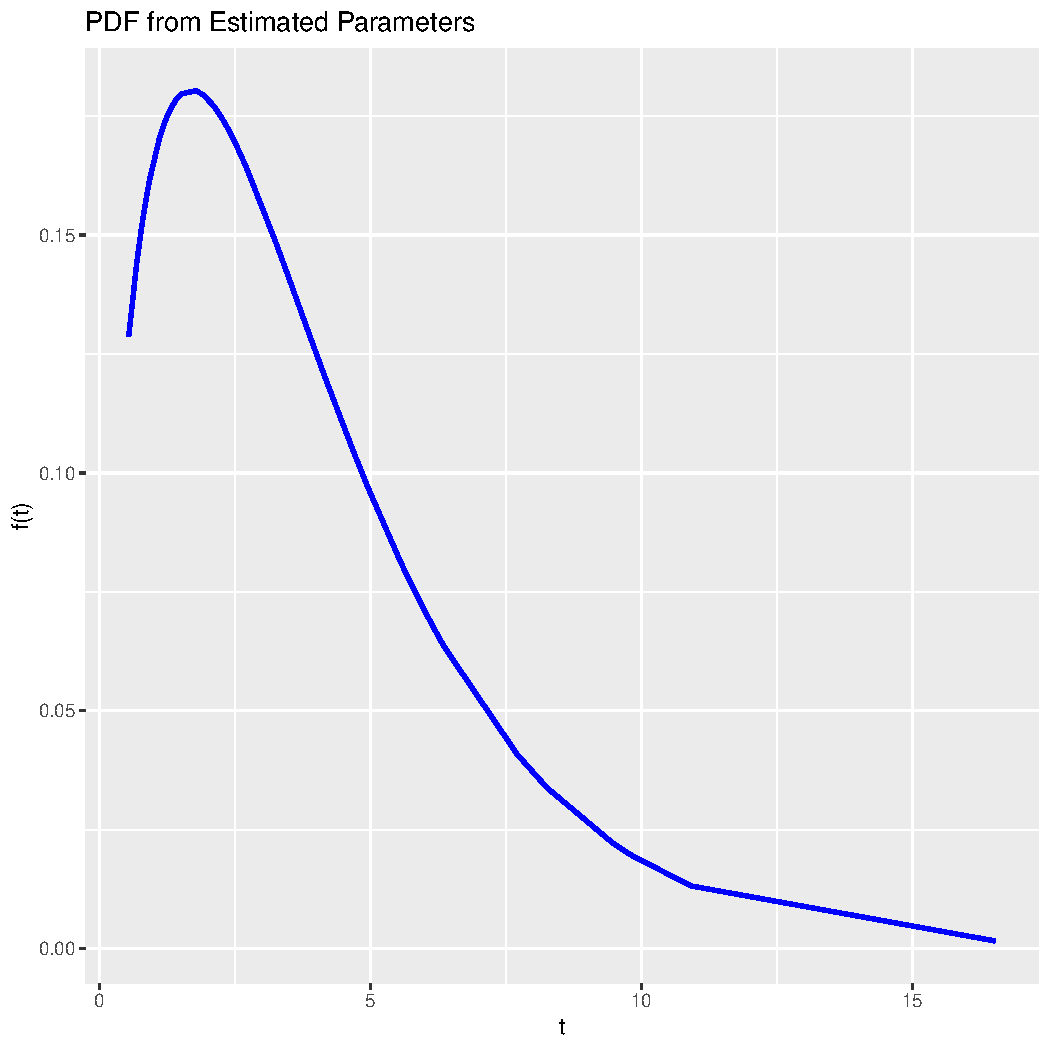
\includegraphics[width=\maxwidth]{figure/unnamed-chunk-7-1} 
\end{knitrout}

\newpage

\begin{knitrout}
\definecolor{shadecolor}{rgb}{0.969, 0.969, 0.969}\color{fgcolor}\begin{kframe}
\begin{alltt}
\hldef{df2} \hlkwb{<-} \hlkwd{data.frame}\hldef{(}\hlkwc{t} \hldef{= t_values,}
                  \hlkwc{Ft} \hldef{=} \hlkwd{pgamma}\hldef{(t_values,} \hlkwc{shape} \hldef{= estimated_shape,}
                              \hlkwc{scale} \hldef{= estimated_scale))}

\hldef{df2} \hlopt
  \hlkwd{ggplot}\hldef{(}\hlkwd{aes}\hldef{(}\hlkwc{x} \hldef{= t,} \hlkwc{y} \hldef{= Ft))} \hlopt{+}
  \hlkwd{geom_line}\hldef{(}\hlkwc{col} \hldef{=} \hlsng{'blue'}\hldef{,} \hlkwc{linewidth} \hldef{=} \hlnum{1}\hldef{)} \hlopt{+}
  \hlkwd{labs}\hldef{(}\hlkwc{x} \hldef{=} \hlsng{"t"}\hldef{,} \hlkwc{y} \hldef{=} \hlsng{"F(t)"}\hldef{,} \hlkwc{title} \hldef{=} \hlsng{"CDF from Estimated Parameters"}\hldef{)}
\end{alltt}
\end{kframe}
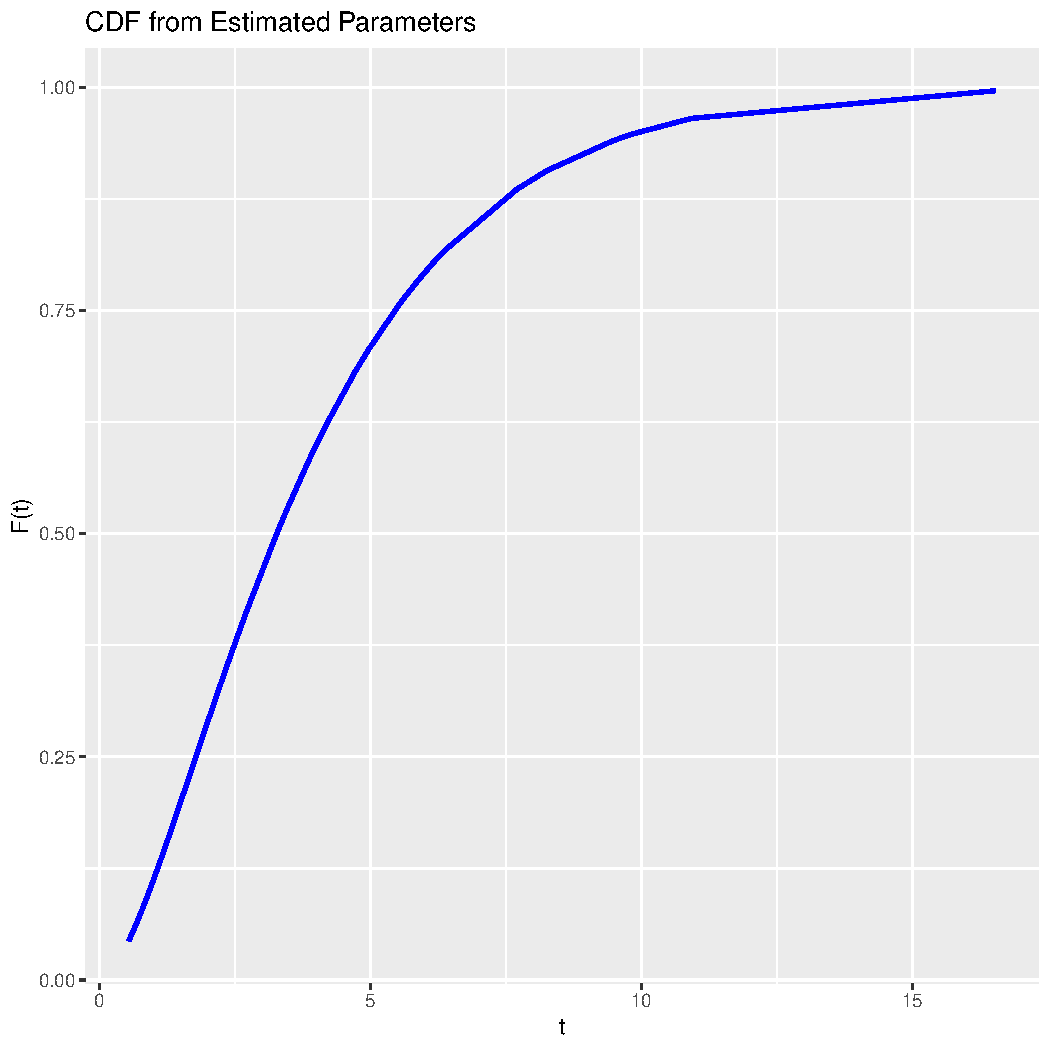
\includegraphics[width=\maxwidth]{figure/unnamed-chunk-8-1} 
\end{knitrout}

\newpage

\begin{knitrout}
\definecolor{shadecolor}{rgb}{0.969, 0.969, 0.969}\color{fgcolor}\begin{kframe}
\begin{alltt}
\hldef{df3} \hlkwb{<-} \hlkwd{data.frame}\hldef{(}\hlkwc{t} \hldef{= t_values,}
                  \hlkwc{St} \hldef{=} \hlnum{1} \hlopt{-} \hlkwd{pgamma}\hldef{(t_values,} \hlkwc{shape} \hldef{= estimated_shape,}
                                  \hlkwc{scale} \hldef{= estimated_scale))}

\hldef{df3} \hlopt
  \hlkwd{ggplot}\hldef{(}\hlkwd{aes}\hldef{(}\hlkwc{x} \hldef{= t,} \hlkwc{y} \hldef{= St))} \hlopt{+}
  \hlkwd{geom_line}\hldef{(}\hlkwc{col} \hldef{=} \hlsng{'blue'}\hldef{,} \hlkwc{linewidth} \hldef{=} \hlnum{1}\hldef{)} \hlopt{+}
  \hlkwd{labs}\hldef{(}\hlkwc{x} \hldef{=} \hlsng{"t"}\hldef{,} \hlkwc{y} \hldef{=} \hlsng{"S(t)"}\hldef{,} \hlkwc{title} \hldef{=} \hlsng{"Survival Function from Estimated Parameters"}\hldef{)}
\end{alltt}
\end{kframe}
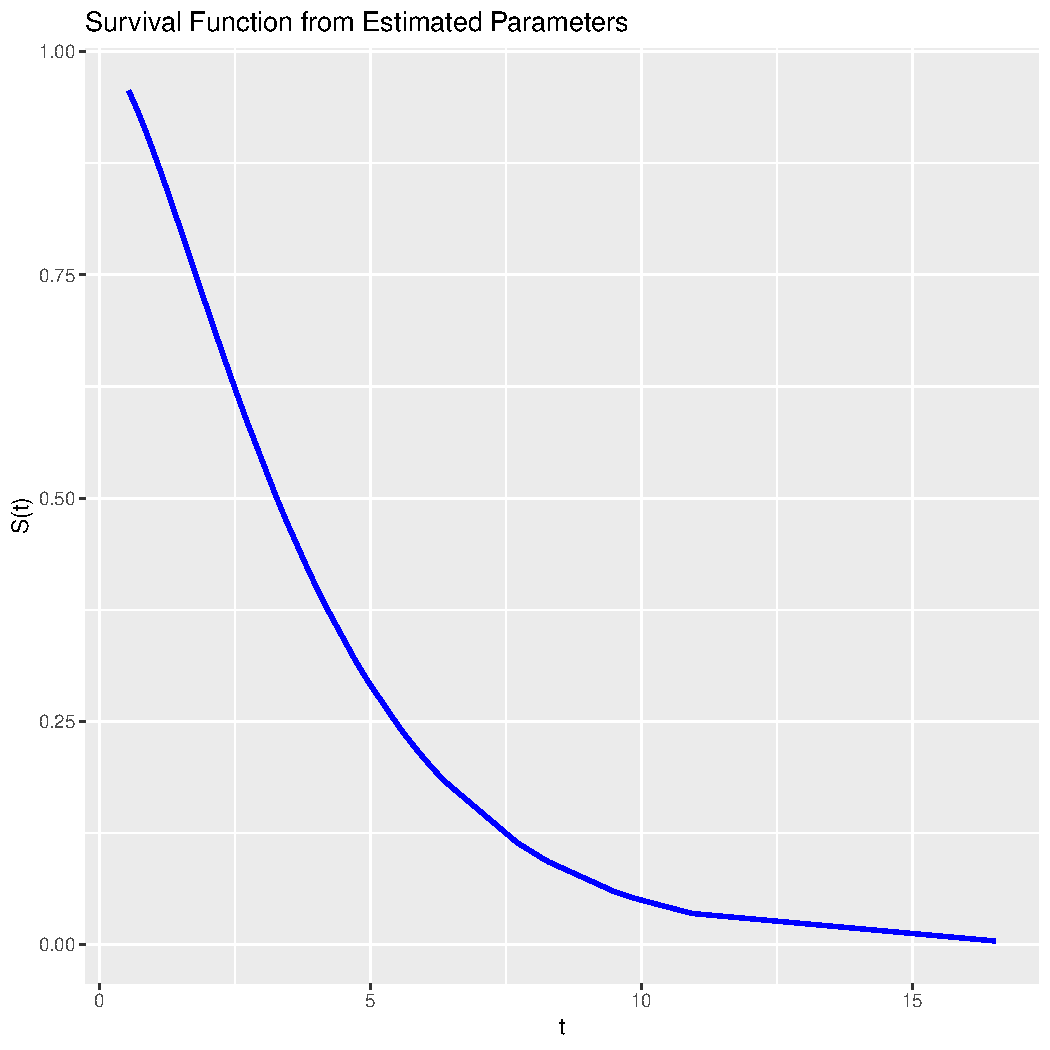
\includegraphics[width=\maxwidth]{figure/unnamed-chunk-9-1} 
\end{knitrout}

\newpage

\begin{knitrout}
\definecolor{shadecolor}{rgb}{0.969, 0.969, 0.969}\color{fgcolor}\begin{kframe}
\begin{alltt}
\hldef{df4} \hlkwb{<-} \hlkwd{data.frame}\hldef{(}\hlkwc{t} \hldef{= t_values,}
                  \hlkwc{ht} \hldef{= df1}\hlopt{$}\hldef{ft} \hlopt{/} \hldef{df3}\hlopt{$}\hldef{St)}

\hldef{df4} \hlopt
  \hlkwd{ggplot}\hldef{(}\hlkwd{aes}\hldef{(}\hlkwc{x} \hldef{= t,} \hlkwc{y} \hldef{= ht))} \hlopt{+}
  \hlkwd{geom_line}\hldef{(}\hlkwc{col} \hldef{=} \hlsng{'blue'}\hldef{,} \hlkwc{linewidth} \hldef{=} \hlnum{1}\hldef{)} \hlopt{+}
  \hlkwd{labs}\hldef{(}\hlkwc{x} \hldef{=} \hlsng{"t"}\hldef{,} \hlkwc{y} \hldef{=} \hlsng{"h(t)"}\hldef{,} \hlkwc{title} \hldef{=} \hlsng{"Hazard Function from Estimated Parameters"}\hldef{)}
\end{alltt}
\end{kframe}
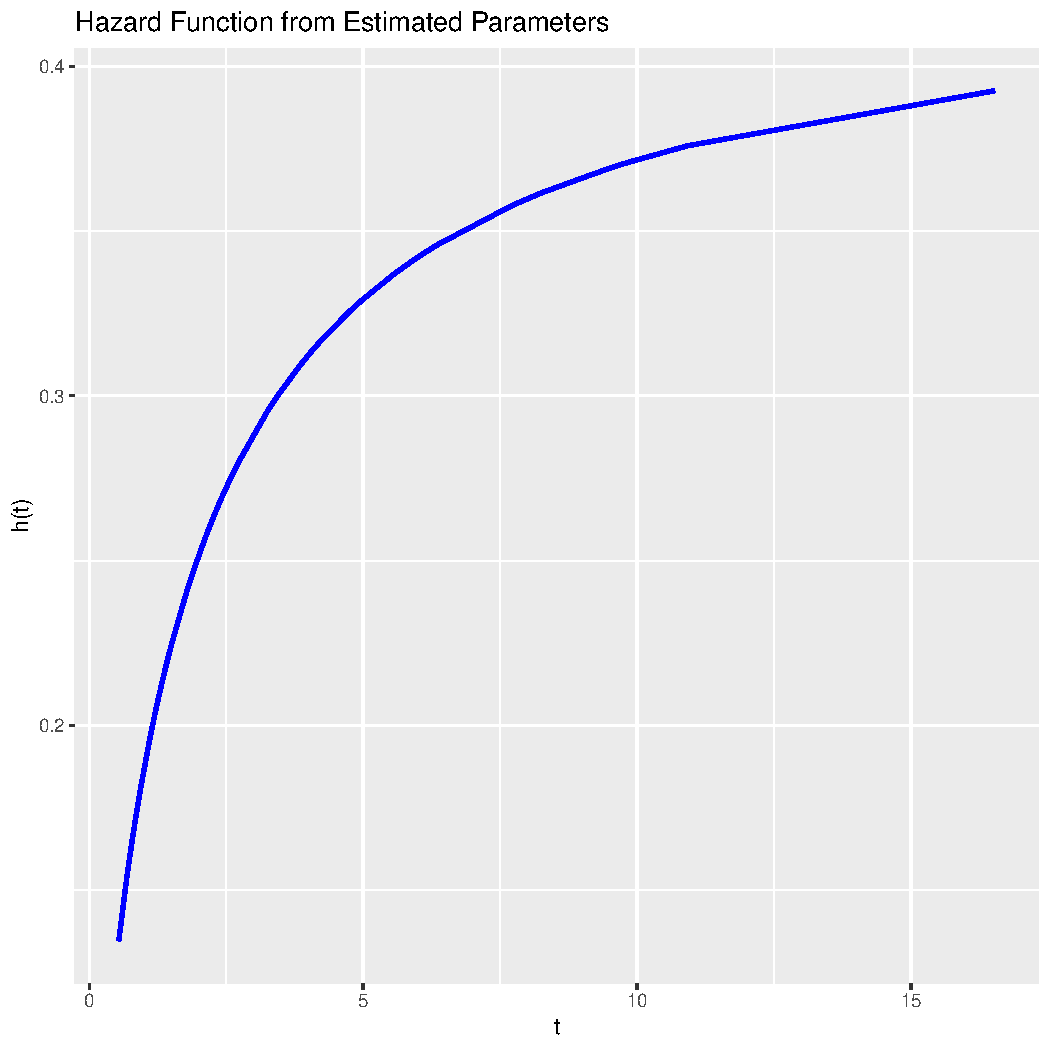
\includegraphics[width=\maxwidth]{figure/unnamed-chunk-10-1} 
\end{knitrout}

\smallpencil \hspace{0.5cm} {\setlength{\spaceskip}{1em plus 0.5em minus 0.5em} \fontsize{17}{20}\myfont For shape parameter less than 1, the hazard function decreases monotonically. \par}

\newpage

\begin{knitrout}
\definecolor{shadecolor}{rgb}{0.969, 0.969, 0.969}\color{fgcolor}\begin{kframe}
\begin{alltt}
\hldef{df5} \hlkwb{<-} \hlkwd{data.frame}\hldef{(}\hlkwc{t} \hldef{= t_values,}
                  \hlkwc{Ht} \hldef{=} \hlopt{-}\hlkwd{log}\hldef{(df3}\hlopt{$}\hldef{St))}

\hldef{df5} \hlopt
  \hlkwd{ggplot}\hldef{(}\hlkwd{aes}\hldef{(}\hlkwc{x} \hldef{= t,} \hlkwc{y} \hldef{= Ht))} \hlopt{+}
  \hlkwd{geom_line}\hldef{(}\hlkwc{col} \hldef{=} \hlsng{'blue'}\hldef{,} \hlkwc{linewidth} \hldef{=} \hlnum{1}\hldef{)} \hlopt{+}
  \hlkwd{labs}\hldef{(}\hlkwc{x} \hldef{=} \hlsng{"t"}\hldef{,} \hlkwc{y} \hldef{=} \hlsng{"H(t)"}\hldef{,}
       \hlkwc{title} \hldef{=} \hlsng{"Cumulative Hazard Function from Estimated Parameters"}\hldef{)}
\end{alltt}
\end{kframe}
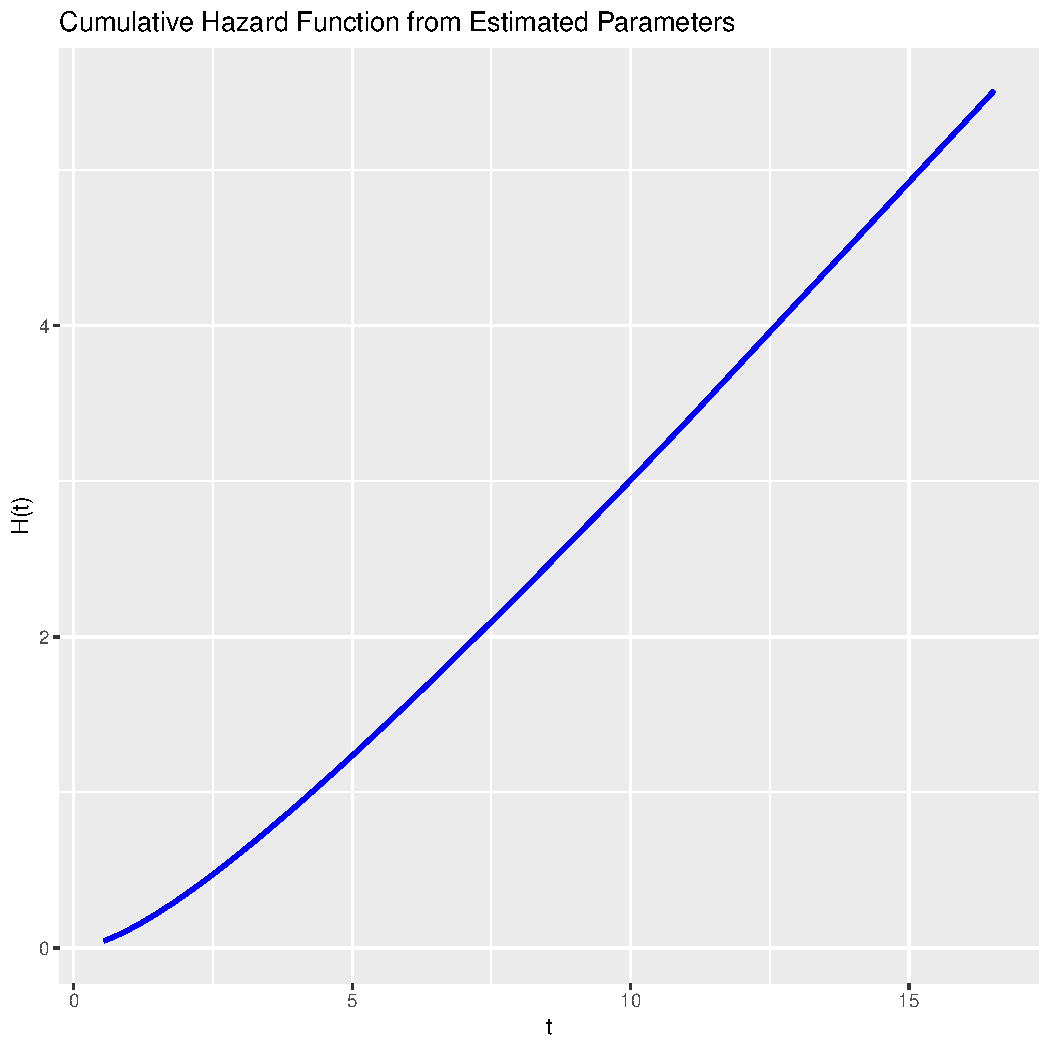
\includegraphics[width=\maxwidth]{figure/unnamed-chunk-11-1} 
\end{knitrout}

\end{document}
